\subsection{The method of characteristics}
\label{m:sec:moc}

The generating-function equations assembled so far --- \cref{m:eq:bdpde} for the
birth--death process, \cref{m:eq:tibdpde} for its time-inhomogeneous version,
\cref{m:eq:bdcpde} for birth--death--catastrophe --- all have the same shape: a
first-order linear partial differential equation whose coefficients do not
involve the unknown. Such equations are solved by the method of
characteristics, and this subsection sets the method out in a form that the
rest of the thesis can use as a recipe, then works one example through to the
end. The remaining members of the family --- the absorption-only model, and the
absorption--birth--death model whose closed form is an original result of this
thesis --- are solved in \cref{m:app:moc} by the identical procedure.

\subsubsection{The recipe}
\label{m:sec:mocrecipe}

Consider a first-order equation for $G$ in two state variables and time,
\begin{equation}
\label{m:eq:generalpde}
\pddt{G} = a(x,y,t)\,\pdd{G}{x} + b(x,y,t)\,\pdd{G}{y},
\qquad
G(x,y,0) = G_0(x,y),
\end{equation}
which is the form every generating-function equation in this thesis takes once
the master equation has been summed. The idea is to find curves
$(x(\tau),y(\tau),t(\tau))$ along which $G$ is constant, so that the PDE
collapses to an ordinary differential equation --- in fact, to nothing at all
--- on each curve. Introduce a parameter $\tau$ along the curves and demand
\begin{equation}
\label{m:eq:charsys}
\dda{G}{\tau} = 0,
\qquad
\dda{t}{\tau} = -1,
\qquad
\dda{x}{\tau} = a,
\qquad
\dda{y}{\tau} = b ,
\end{equation}
with initial data anchored on the surface $t=0$:
\begin{equation}
\label{m:eq:ICpar}
x(\sigma,\eta,0)=\sigma,
\qquad
y(\sigma,\eta,0)=\eta,
\qquad
t(\sigma,\eta,0)=0 .
\end{equation}
The choice $\dd t/\dd\tau=-1$ makes $\tau=-t$, so characteristics run
\emph{backwards} in time from any point $(x,y,t)$ down to the initial surface;
that is what allows the initial condition to be read off at the end. The recipe
is then:
\begin{enumerate}[label=\textup{(\arabic*)}]
\item solve the characteristic ODEs in \cref{m:eq:charsys} with the anchoring
\cref{m:eq:ICpar};
\item since $G$ is constant along each characteristic,
$G = G_0(\sigma,\eta)$ everywhere on it;
\item eliminate $(\sigma,\eta,\tau)$ in favour of $(x,y,t)$ by inverting the
solutions of step \textup{(1)};
\item substitute into $G_0$ to obtain $G(x,y,t)$.
\end{enumerate}
Everything in step \textup{(3)} is algebra; the entire difficulty of any
particular problem lives in step \textup{(1)}, where the characteristic ODE for
$x$ may be nonlinear. When it is a Riccati equation, as it is for every
birth--death-type model in this thesis, it factorises and separates; when the
coefficients depend on $t$, as in \cref{m:eq:tibdpde}, the same steps go
through with $t$-dependent right-hand sides.

\subsubsection{Worked example: absorption--death}
\label{m:sec:mocabsdeath}

A compartment takes up particles from a surrounding medium, and particles
already inside it may die. Let $X_t$ and $Y_t$ count the particles inside and
outside the compartment, started from $X_0=0$, $Y_0=N$. Absorption occurs at
rate $\alpha$ per exterior particle and death at rate $\mu$ per interior
particle; both remove a particle from further consideration, so every particle
ends either inside, outside, or dead, and no count can exceed $N$. The
transition probabilities over an infinitesimal interval are
\begin{align*}
\pr{\Delta X = 1,\ \Delta Y = -1} &= \alpha j\,\Delta t, &&\text{(absorption)}\\
\pr{\Delta X = -1} &= \mu i\,\Delta t, &&\text{(death)}\\
\pr{\Delta X = 0,\ \Delta Y = 0} &= 1-(\alpha j+\mu i)\Delta t, &&\text{(no event)}
\end{align*}
with forward Kolmogorov equations
\begin{equation}
\label{m:eq:FK2}
\ddt{p_{i,j}} = \alpha(j+1)p_{i-1,j+1} + \mu(i+1)p_{i+1,j} - (\alpha j+\mu i)p_{i,j} .
\end{equation}
Multiplying by $x^iy^j$, summing, and shifting indices as in \cref{m:sec:pgf}
gives the generating-function equation, in exactly the form
\cref{m:eq:generalpde}:
\begin{equation}
\label{m:eq:PDE2}
\pddt{G} = \mu(1-x)\pdd{G}{x} + \alpha(x-y)\pdd{G}{y},
\qquad G(x,y,0) = y^N .
\end{equation}

\paragraph{Step 1: the characteristic ODEs.}
From \cref{m:eq:charsys} with $a=\mu(1-x)$ and $b=\alpha(x-y)$,
\begin{align}
\dda{G}{\tau} &= 0, \label{m:eq:ch11}\\
\dda{t}{\tau} &= -1, \label{m:eq:ch12}\\
\dda{x}{\tau} &= \mu(1-x), \label{m:eq:ch13}\\
\dda{y}{\tau} &= \alpha(x-y). \label{m:eq:ch14}
\end{align}
\Cref{m:eq:ch12} gives $t=-\tau$ at once. \Cref{m:eq:ch13} separates:
$1-x = (1-\sigma)\ee^{-\mu\tau}$. Substituting that into \cref{m:eq:ch14} and
solving with the integrating factor $\ee^{\alpha\tau}$,
\begin{equation*}
y = 1-\frac{\alpha}{\alpha-\mu}(1-\sigma)\ee^{-\mu\tau}
+ c(\sigma,\eta)\ee^{-\alpha\tau},
\end{equation*}
and the anchoring \cref{m:eq:ICpar} fixes
$c(\sigma,\eta) = \eta + \frac{\alpha}{\alpha-\mu}(1-\sigma)-1$, so
\begin{equation}
\label{m:eq:ywitheta}
y = 1-\frac{\alpha}{\alpha-\mu}(1-\sigma)\ee^{-\mu\tau}
+ \lrb{\eta + \frac{\alpha}{\alpha-\mu}(1-\sigma)-1}\ee^{-\alpha\tau} .
\end{equation}

\paragraph{Steps 2--3: constant on characteristics, then inversion.}
By \cref{m:eq:ch11}, $G$ equals its initial value on each characteristic, and
under \cref{m:eq:ICpar} the initial condition reads $G_0(\sigma,\eta)=\eta^N$:
\begin{equation}
\label{m:eq:GetaN}
G = \eta^N .
\end{equation}
It remains to express $\eta$ in terms of $(x,y,t)$. Rearranging
\cref{m:eq:ywitheta} for $\eta$, substituting $1-\sigma=(1-x)\ee^{\mu\tau}$
from the $x$-solution and $\tau=-t$, gives after simplification
\begin{equation*}
\eta = 1-\frac{\mu}{\mu-\alpha}\ee^{-\alpha t}
+ \frac{\alpha}{\mu-\alpha}\ee^{-\mu t}
+ \frac{\alpha}{\mu-\alpha}\bigl(\ee^{-\alpha t}-\ee^{-\mu t}\bigr)x
+ \ee^{-\alpha t}y .
\end{equation*}

\paragraph{Step 4: the generating function.}
Substituting into \cref{m:eq:GetaN},
\begin{equation}
\label{m:eq:Gabsdeath}
G(x,y,t) = \Bigl(
1-\tfrac{\mu}{\mu-\alpha}\ee^{-\alpha t} + \tfrac{\alpha}{\mu-\alpha}\ee^{-\mu t}
+ \tfrac{\alpha}{\mu-\alpha}\bigl(\ee^{-\alpha t}-\ee^{-\mu t}\bigr)x
+ \ee^{-\alpha t}y\Bigr)^N ,
\end{equation}
with the removable degeneracy $\alpha=\mu$ understood by its limit,
\begin{equation}
\label{m:eq:equalrates}
\frac{\alpha}{\mu-\alpha}\bigl(\ee^{-\alpha t}-\ee^{-\mu t}\bigr)
\;\xrightarrow[\mu\to\alpha]{}\;
\alpha t\,\ee^{-\alpha t} .
\end{equation}

\paragraph{The check.}
Because particles neither interact nor multiply in this model, the answer can
be obtained independently, and the two routes should agree. A single particle
has state probabilities
\begin{equation}
\label{m:eq:absdeathstates}
p_{0,1}(t) = \ee^{-\alpha t},
\qquad
p_{1,0}(t) = \frac{\alpha}{\mu-\alpha}\lrb{\ee^{-\alpha t}-\ee^{-\mu t}},
\qquad
p_{0,0}(t) = 1-p_{0,1}(t)-p_{1,0}(t),
\end{equation}
outside, inside and dead respectively (\cref{m:fig:abs2}). The $N$ particles
act independently,
so the joint generating function is the $N$th power of the single-particle one
--- which is precisely the form \cref{m:eq:Gabsdeath}, with the three bracket
terms as the probabilities of dead, inside and outside. Setting $x=y=1$
confirms that the three probabilities sum to one, and setting $x=1$ alone gives
$G(1,y,t) = (\ee^{-\alpha t}y + 1-\ee^{-\alpha t})^N$: the exterior count is
binomial, as it must be, since exterior particles are absorbed independently at
rate $\alpha$ regardless of what happens inside.

\begin{figure}[ht]
\centering
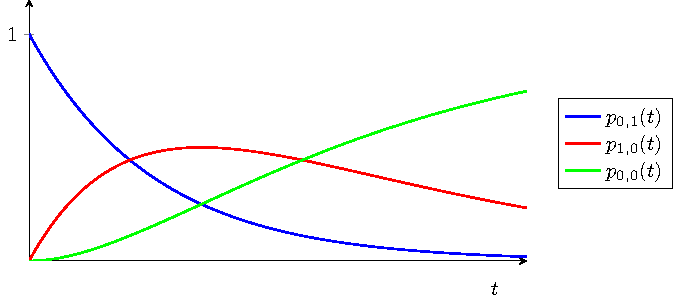
\includegraphics[width=0.62\textwidth]{figures/abs2.pdf}
\caption{State probabilities for a single particle in the absorption--death
model. The particle starts outside (blue, decaying at rate $\alpha$), is
absorbed into the compartment (red, which rises and then decays as death takes
over), and finally dies (green, absorbing). The three curves sum to one at
every time, and the coefficients of \cref{m:eq:Gabsdeath} are read off them.}
\label{m:fig:abs2}
\end{figure}

The same four steps, applied to harder coefficients, produce the remaining
closed forms of this thesis. Adding interior birth to the model above opens an
infinite state space, the independence check fails, and the characteristic
calculation becomes the only route; it is carried out in \cref{m:app:moc},
whose end product --- the absorption--birth--death generating function,
\cref{m:eq:Gabd} --- is the closed form on which the absorption models of later
chapters are built. The two support appendices belong to this subsection as
well: \cref{m:app:hyp} records the hypergeometric integral identity that the
harder calculation rests on, and \cref{m:app:extract} explains how to recover
time-dependent state probabilities from a generating function given by a
formula rather than a series.
